\documentclass[../main.tex]{subfiles}

\begin{document}

\section*{第1問}

{\bf [解]}
\begin{align*}
a_1&=1\quad\cdots①\\
\log a_{n+1}-\log a_n&=\log n-\log(n+2)\quad\cdots②
\end{align*}

②から，$\log\dfrac{a_{n+1}}{a_n}=\log\dfrac n{n+2}\quad\therefore\dfrac{a_{n+1}}{a_n}=\dfrac n{n+2}$（$\because\log x$は単調）

だから，
\begin{align*}
(n+2)a_{n+1}&=na_n\quad\cdots③\\
(n+2)(n+1)a_{n+1}&=(n+1)na_n
\end{align*}

くり返し用いて，
\begin{align*}
(n+1)na_n=2\cdot1\cdot a_1=2\quad(\because①)
\end{align*}
\begin{align*}
\therefore\ a_n=\frac2{n(n+1)}=2\left(\frac1n-\frac1{n+1}\right)
\end{align*}

だから，
\begin{align*}
\sum_{k=1}^na_k=2\left(1-\frac1{n+1}\right)=\frac{2n}{n+1}．
\end{align*}

\newpage

\section*{第2問}

{\bf [解]}
$f(x)=x\sin x\ (x\ge0)$，$f'(x)=\sin x+x\cos x$である．$f'(\pi/2)=1$だから，$x=\pi/2$での法線は$y=-x+\pi$である．

\begin{figure}[htb]
\centering
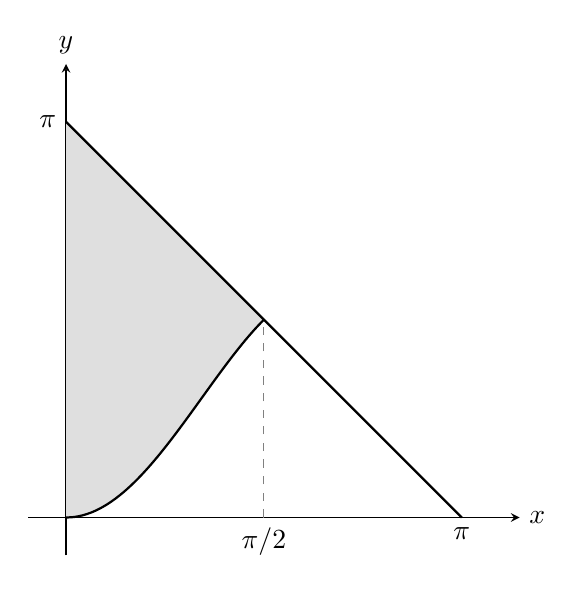
\begin{tikzpicture}[scale=1.6, >=stealth]
  \draw[->] (-0.3,0) -- (3.6,0) node[right] {$x$};
  \draw[->] (0,-0.3) -- (0,3.6) node[above] {$y$};
  \fill[gray!25] plot[domain=0:1.5708, smooth] (\x,{\x*sin(\x r)}) -- (0,3.1416) -- cycle;
  \draw[domain=0:1.5708, smooth, thick] plot (\x,{\x*sin(\x r)});
  \draw[thick] (0,3.1416) -- (3.1416,0);
  \draw[gray, dashed] (1.5708,0) -- (1.5708,1.5708);
  \node[below] at (1.5708,0) {$\pi/2$};
  \node[below] at (3.1416,0) {$\pi$};
  \node[left] at (0,3.1416) {$\pi$};
\end{tikzpicture}
\caption{$y=f(x)$，法線，$y$軸で囲まれる図形（斜線部）}
\end{figure}

これを$x$軸まわりに回転してできる立体の体積は
\begin{align*}
V=\pi\int_0^{\pi/2}\left[(-x+\pi)^2-x^2\sin^2x\right]dx\quad\cdots①
\end{align*}

ここで，
\begin{align*}
\int_0^{\pi/2}x^2\sin^2x\,dx=\int_0^{\pi/2}\frac12x^2(1-\cos2x)\,dx\quad\cdots②
\end{align*}
であり，
\begin{align*}
\int_0^{\pi/2}x^2\cos2x\,dx=\left[\frac{x^2}2\sin2x+\frac{2x}4\cos2x-\frac28\sin2x\right]_0^{\pi/2}=-\frac\pi4
\end{align*}

から，②に代入して
\begin{align*}
\int_0^{\pi/2}x^2\sin^2x\,dx=\frac12\left[\frac13x^3\right]_0^{\pi/2}+\frac\pi8=\frac1{48}\pi^3+\frac18\pi\quad\cdots③
\end{align*}

又，
\begin{align*}
\int_0^{\pi/2}(x-\pi)^2\,dx=\left[\frac13x^3-\pi x^2+\pi^2x\right]_0^{\pi/2}=\frac7{24}\pi^3\quad\cdots④
\end{align*}

③④を①に代入して
\begin{align*}
V&=\pi\left\{\frac7{24}\pi^3-\frac1{48}\pi^3-\frac18\pi\right\}\\
&=\pi\left(\frac{13}{48}\pi^3-\frac18\pi\right)．
\end{align*}

\newpage

\section*{第3問}

{\bf [解]}

\begin{figure}[htb]
\centering
\begin{tikzpicture}[scale=1.6, >=stealth]
  \coordinate (O) at (1.1,2.2);
  \coordinate (A) at (0,0);
  \coordinate (B) at (2.2,0);
  \coordinate (C) at (2.7,1.1);
  \draw (O) -- (A) -- (B) -- (C) -- (O);
  \draw (A) -- (B);
  \draw[dashed] (A) -- (C);
  \draw[dashed] (O) -- (B);
  \node[above] at (O) {$O$};
  \node[below left] at (A) {$A$};
  \node[below right] at (B) {$B$};
  \node[right] at (C) {$C$};
\end{tikzpicture}
\caption{四面体$OABC$}
\end{figure}

点$X$に対し，$\overrightarrow{OX}=\vec x$と定める．(i)から
\begin{align*}
\vec a\cdot(\vec c-\vec b)&=0\\
\vec b\cdot(\vec c-\vec a)&=0\\
\vec c\cdot(\vec b-\vec a)&=0
\end{align*}
$\cdots①$

又，(ii)から，$\triangle OAB$の面積を$T$として，
\begin{align*}
T&=\frac12\sqrt{|\vec a|^2|\vec b|^2-(\vec a\cdot\vec b)^2}\\
&=\frac12\sqrt{|\vec b|^2|\vec c|^2-(\vec b\cdot\vec c)^2}\\
&=\frac12\sqrt{|\vec c|^2|\vec a|^2-(\vec c\cdot\vec a)^2}\\
&=\frac12\sqrt{|\vec b-\vec a|^2|\vec c-\vec a|^2-\{(\vec b-\vec a)\cdot(\vec c-\vec a)\}^2}
\end{align*}
$\cdots②$

である．①から，$\vec a\cdot\vec b=\vec b\cdot\vec c=\vec c\cdot\vec a\ (=q$とする$)\quad\cdots③$だから，第1，2，3辺が等しいことより②から
\begin{align*}
|\vec a|^2|\vec b|^2=|\vec b|^2|\vec c|^2=|\vec c|^2|\vec a|^2\quad\cdots④
\end{align*}
となる．$|\vec a|,|\vec b|,|\vec c|>0$から，
\begin{align*}
|\vec a|=|\vec b|=|\vec c|\ (=p\ \text{とする})\quad\cdots⑤
\end{align*}

である．さらに②から
\begin{align*}
T&=\frac12\sqrt{4(p^2-q)^2-(p^2-q)^2}\\
&=\frac12\sqrt{p^4-q^2}
\end{align*}

$y=x^2$は単調増加だから，$T$の中身を比較して，
\begin{align*}
4(p^2-q)^2-(p^2-q)^2&=p^4-q^2\\
3(p^2-q)^2&=p^4-q^2\\
2p^4-6p^2q+4q^2&=0\\
(p^2-2q)(2p^2-2q)&=0
\end{align*}
\begin{align*}
\therefore\ q=\frac12p^2,\ p^2\quad\cdots⑥
\end{align*}

ところで，$\angle AOB=\alpha$とすれば，$q=p^2\cos\alpha$であり，$0<\alpha<\pi$（$\because$退化しない四面体）のため$|q|<p^2$だから，⑥で$q=\dfrac12p^2$が正しい．この時
\begin{align*}
|\vec a-\vec b|=|\vec b-\vec c|=|\vec c-\vec a|=\sqrt{2p^2-p^2}=p\quad(\because\text{各項}0\text{以上})\quad\cdots⑦
\end{align*}

である．⑤⑦から，四面体$OABC$は各辺の長さが等しく，正四面体である．$\blacksquare$

\bigskip
\noindent{\bf [別解]}
（⑥以下）同様に，頂点を$O$から$A$，$B$，$C$にとり直すことにより，
\begin{align*}
|\overrightarrow{AB}|=|\overrightarrow{BC}|=|\overrightarrow{CA}|=|\overrightarrow{OA}|\quad\cdots⑧
\end{align*}
を得る．⑤⑧から示された．$\blacksquare$

\newpage

\section*{第4問}

{\bf [解]}
$x^2+x+1=0$の2解を$\omega,\bar\omega$とおくと，$\omega=\dfrac{-1+\sqrt3i}2$より$\bar\omega=\omega^2$である．又，$\omega^3=1$である．$F(x)=(x^{100}+1)^{100}+(x^2+1)^{100}+1$とおく．
\begin{align*}
F(\omega)&=(\omega+1)^{100}+(-\omega)^{100}+1\\
&=(-\omega^2)^{100}+\omega+1\\
&=\omega^2+\omega+1=0
\end{align*}
\begin{align*}
F(\omega^2)&=(\omega^2+1)^{100}+(\omega+1)^{100}+1\\
&=(-\omega)^{100}+(-\omega^2)^{100}+1\\
&=\omega^2+\omega+1=0
\end{align*}

より，因数定理から，$F(x)$は$x^2+x+1$で割り切れる．$\blacksquare$

\newpage

\section*{第5問}

% (原稿において第5問の解答は空欄)
\newpage

\section*{第6問}

{\bf [解]}
$n$チームを$a_k$（$k=1,2,\ldots,n$）とおく．$n-2$勝$1$敗の$2$チームの選び方は${}_n\mathrm C_2=\dfrac{n(n-1)}2$通りである．以下，この$2$チームが$a_1,a_2$の時を考える．対称性から，$a_1$が$a_2$に勝つ時を考える．$\cdots①$

この時，考える対戦結果は次のようになる：$a_1$は$a_2$に勝ち，$a_3,\ldots,a_n$のうちある$1$チーム$a_k$（$3\le k\le n$）にのみ負ける．$a_2$は$a_1$に負け，$a_3,\ldots,a_n$には全て勝つ．

この時，$a_1$は$a_k$にのみ負ける（$3\le k\le n$）．$a_2$は$a_3$〜$a_n$に全て勝つ．したがって，$a_3$〜$a_n$の中で，$a_k$以外は必ず$2$敗する．$a_k$が$2$敗以上する確率は$1-\left(\dfrac12\right)^{n-3}$（$\because$排反）だから，のこる確率は
\begin{align*}
\left(\frac12\right)^{2n-3}\left\{1-\left(\frac12\right)^{n-3}\right\}
\end{align*}

したがって，$a_1,a_2$が$(n-2)$勝$1$敗となる確率$P$は
\begin{align*}
P&=(n-2)\cdot2\left(\frac12\right)^{2n-3}\left\{1-\left(\frac12\right)^{n-3}\right\}\\
&=(n-2)\left(\frac12\right)^{2n-4}\left\{1-\left(\frac12\right)^{n-3}\right\}
\end{align*}

だから，全ての場合について足して，
\begin{align*}
n(n-1)(n-2)\left(\frac12\right)^{2n-3}\left\{1-\left(\frac12\right)^{n-3}\right\}．
\end{align*}

\newpage

\end{document}
